

\newtoggle{inTableHeader}% Track if still in header of table
\toggletrue{inTableHeader}% Set initial value
\newcommand*{\StartTableHeader}{\global\toggletrue{inTableHeader}}%
\newcommand*{\EndTableHeader}{\global\togglefalse{inTableHeader}}%

% Redefine tabular to initialize \StartTableHeader at start and end
\let\OldTabular\tabular%
\let\OldEndTabular\endtabular%
\renewenvironment{tabular}{\StartTableHeader\OldTabular}{\OldEndTabular\StartTableHeader}%

 %The min, mid and max values
\newcommand*{\MinNumberA}{0.5}%
\newcommand*{\MidNumberA}{0.75}%
\newcommand*{\MaxNumberA}{1.0}%

%Apply the gradient macro
\newcommand{\ApplyGradientA}[1]{%
    %\IfDecimal{#1}{
  \iftoggle{inTableHeader}{#1}{
    \ifdim #1 pt > \MidNumberA pt
        \pgfmathsetmacro{\PercentColor}{max(min(100.0*(#1 - \MidNumberA)/(\MaxNumberA-\MidNumberA),100.0),0.00)} %
        \colorbox{green!\PercentColor!yellow}{#1}
    \else
        \pgfmathsetmacro{\PercentColor}{max(min(100.0*(\MidNumberA - #1)/(\MidNumberA-\MinNumberA),100.0),0.00)} %
        \colorbox{red!\PercentColor!yellow}{#1}
    \fi
  }
  %}{#1}
  }


 %The min, mid and max values
\newcommand*{\MinNumberB}{0.0}%
\newcommand*{\MidNumberB}{0.05}%
\newcommand*{\MaxNumberB}{0.1}%
  
%Apply the gradient macro
\newcommand{\ApplyGradientB}[1]{%
    %\IfDecimal{#1}{
  \iftoggle{inTableHeader}{#1}{
    \ifdim #1 pt > \MidNumberB pt
        \pgfmathsetmacro{\PercentColor}{max(min(100.0*(#1 - \MidNumberB)/(\MaxNumberB-\MidNumberB),100.0),0.00)} %
        \colorbox{red!\PercentColor!yellow}{#1}
    \else
        \pgfmathsetmacro{\PercentColor}{max(min(100.0*(\MidNumberB - #1)/(\MidNumberB-\MinNumberB),100.0),0.00)} %
        \colorbox{green!\PercentColor!yellow}{#1}
    \fi
  }
  %}{#1}
  }

%The min, mid and max values
\newcommand*{\MinNumberC}{0.5}%
\newcommand*{\MidNumberC}{0.75}%
\newcommand*{\MaxNumberC}{1.0}%
  
%Apply the gradient macro
\newcommand{\ApplyGradientC}[1]{%
    %\IfDecimal{#1}{
  \iftoggle{inTableHeader}{#1}{
    \ifdim #1 pt > \MidNumberC pt
        \pgfmathsetmacro{\PercentColor}{max(min(100.0*(#1 - \MidNumberC)/(\MaxNumberC-\MidNumberC),100.0),0.00)} %
        \colorbox{green!\PercentColor!yellow}{#1}
    \else
        \pgfmathsetmacro{\PercentColor}{max(min(100.0*(\MidNumberC - #1)/(\MidNumberC-\MinNumberC),100.0),0.00)} %
        \colorbox{red!\PercentColor!yellow}{#1}
    \fi
  }
  %}{#1}
  }

  
 %The min, mid and max values
\newcommand*{\MinNumberD}{0.5}%
\newcommand*{\MidNumberD}{0.75}%
\newcommand*{\MaxNumberD}{1.0}%

%Apply the gradient macro
\newcommand{\ApplyGradientD}[1]{%
    %\IfDecimal{#1}{
  \iftoggle{inTableHeader}{#1}{
    \ifdim #1 pt > \MidNumberD pt
        \pgfmathsetmacro{\PercentColor}{max(min(100.0*(#1 - \MidNumberD)/(\MaxNumberD-\MidNumberD),100.0),0.00)} %
        \colorbox{green!\PercentColor!yellow}{#1}
    \else
        \pgfmathsetmacro{\PercentColor}{max(min(100.0*(\MidNumberD - #1)/(\MidNumberD-\MinNumberD),100.0),0.00)} %
        \colorbox{red!\PercentColor!yellow}{#1}
    \fi
  }
  %}{#1}
  }
   %The min, mid and max values
\newcommand*{\MinNumberE}{0.5}%
\newcommand*{\MidNumberE}{0.75}%
\newcommand*{\MaxNumberE}{1.0}%

%Apply the gradient macro
\newcommand{\ApplyGradientE}[1]{%
    %\IfDecimal{#1}{
  \iftoggle{inTableHeader}{#1}{
    \ifdim #1 pt > \MidNumberE pt
        \pgfmathsetmacro{\PercentColor}{max(min(100.0*(#1 - \MidNumberE)/(\MaxNumberE-\MidNumberE),100.0),0.00)} %
        \colorbox{green!\PercentColor!yellow}{#1}
    \else
        \pgfmathsetmacro{\PercentColor}{max(min(100.0*(\MidNumberE - #1)/(\MidNumberE-\MinNumberE),100.0),0.00)} %
        \colorbox{red!\PercentColor!yellow}{#1}
    \fi
  }
  %}{#1}
  }
     %The min, mid and max values
\newcommand*{\MinNumberF}{0.5}%
\newcommand*{\MidNumberF}{0.75}%
\newcommand*{\MaxNumberF}{1.0}%

%Apply the gradient macro
\newcommand{\ApplyGradientF}[1]{%
    %\IfDecimal{#1}{
  \iftoggle{inTableHeader}{#1}{
    \ifdim #1 pt > \MidNumberF pt
        \pgfmathsetmacro{\PercentColor}{max(min(100.0*(#1 - \MidNumberF)/(\MaxNumberF-\MidNumberF),100.0),0.00)} %
        \colorbox{green!\PercentColor!yellow}{#1}
    \else
        \pgfmathsetmacro{\PercentColor}{max(min(100.0*(\MidNumberF - #1)/(\MidNumberF-\MinNumberF),100.0),0.00)} %
        \colorbox{red!\PercentColor!yellow}{#1}
    \fi
  }
  %}{#1}
  }
     %The min, mid and max values
\newcommand*{\MinNumberG}{0.5}%
\newcommand*{\MidNumberG}{0.75}%
\newcommand*{\MaxNumberG}{1.0}%

%Apply the gradient macro
\newcommand{\ApplyGradientG}[1]{%
    %\IfDecimal{#1}{
  \iftoggle{inTableHeader}{#1}{
    \ifdim #1 pt > \MidNumberG pt
        \pgfmathsetmacro{\PercentColor}{max(min(100.0*(#1 - \MidNumberG)/(\MaxNumberG-\MidNumberG),100.0),0.00)} %
        \colorbox{green!\PercentColor!yellow}{#1}
    \else
        \pgfmathsetmacro{\PercentColor}{max(min(100.0*(\MidNumberG - #1)/(\MidNumberG-\MinNumberG),100.0),0.00)} %
        \colorbox{red!\PercentColor!yellow}{#1}
    \fi
  }
  %}{#1}
  }
     %The min, mid and max values
\newcommand*{\MinNumberH}{0.5}%
\newcommand*{\MidNumberH}{0.75}%
\newcommand*{\MaxNumberH}{1.0}%

%Apply the gradient macro
\newcommand{\ApplyGradientH}[1]{%
    %\IfDecimal{#1}{
  \iftoggle{inTableHeader}{#1}{
    \ifdim #1 pt > \MidNumberH pt
        \pgfmathsetmacro{\PercentColor}{max(min(100.0*(#1 - \MidNumberH)/(\MaxNumberH-\MidNumberH),100.0),0.00)} %
        \colorbox{green!\PercentColor!yellow}{#1}
    \else
        \pgfmathsetmacro{\PercentColor}{max(min(100.0*(\MidNumberH - #1)/(\MidNumberH-\MinNumberH),100.0),0.00)} %
        \colorbox{red!\PercentColor!yellow}{#1}
    \fi
  }
  %}{#1}
  }



\newcolumntype{A}{>{\collectcell\ApplyGradientA}c<{\endcollectcell}}
\newcolumntype{B}{>{\collectcell\ApplyGradientB}c<{\endcollectcell}}
\newcolumntype{C}{>{\collectcell\ApplyGradientC}c<{\endcollectcell}}
\newcolumntype{D}{>{\collectcell\ApplyGradientD}c<{\endcollectcell}}
\newcolumntype{E}{>{\collectcell\ApplyGradientE}c<{\endcollectcell}}
\newcolumntype{F}{>{\collectcell\ApplyGradientF}c<{\endcollectcell}}
\newcolumntype{G}{>{\collectcell\ApplyGradientG}c<{\endcollectcell}}
\newcolumntype{H}{>{\collectcell\ApplyGradientH}c<{\endcollectcell}}

\renewcommand{\arraystretch}{1}
\setlength{\fboxsep}{2mm} % box size
\setlength{\tabcolsep}{-4pt}

\chapter{Výsledky}
\label{kap:results}

V tejto kapitole odprezentujeme výsledky dosiahnuté pri triangulácii končných aj 
nekonečných, neohraničených plôch. Označme počet trojuholníkov vo výslednej triangulácii 
ako $n$ a počet vrcholov $p$.

\section{Kritéria kvality výslednej triangulácie}
\begin{enumerate}
\item{
    \textit{Priemerná dĺžka hrany}

    Pri zmenšovaní hrany vznikajú body $x_{proj}$ bližšie k povrchu, preto je ich premietnutie
    presnejšia. Vzniknuté premietnuté trojuholníky majú preto dĺžku hrany bližšiu k zadanej dĺžke 
    $a$. Pre naše modely odmeriame priemernú dĺžku hrany a porovnáme ju so zadanou dĺžkou hrany $a$. 
    Dané porovnanie vyjadríme 
    pomerom, na ktorom budeme sledovať, či sa pri zmenšujúcej zadanej dĺžke $a$ približuje k $1$.

    Kritérium budeme označovať $k_1$.
}
\item{
    \textit{Vzdialenosť ťažiska od kolmého priemetu ťažiska}

    Zmenšovaním veľkosti hrany by sa mala priemerná vzdialenosť ťažiska od svojho kolmého 
    priemetu zmenšovať. Odmeriame a budeme sledovať, či sa daná priemerná vzdialenosť
    zmenšuje pri zmenšovaní dĺžky hrany $a$. Takisto budeme sledovať aj pomer priemernej 
    vzdialenosti a zadanej dĺžky hrany $a$. Ak sa tento pomer pri zmenšujúcej sa dĺžke hrany 
    $a$ zmenšuje, vzdialenosť 
    ťažiska od svojho priemetu klesá rýchlejšie ako dĺžka zadanej hrany $a$.

    Kritérium budeme označovať $k_2$.
}
\item{
    \textit{Pomer dĺžok strán trojuholníka}

    Zmenšovaním veľkosti hrany by malo vznikať viac takmer rovnostranných trojuholníkov.
    Dôvodom je, že menšie trojuholníky dokážu plochu presnejšie aproximovať aj v oblastiach 
    s väčším zakrivením. Preto sa trojuholníky nemusia nevhodne spájať a vytvárať množstvo 
    úzkych trojuholníkov. Opísanú vlastnosť budeme merať ako pomer dĺžok strán trojuholníka. 
    
    Majme trojuholník $T(x_i, x_j, x_k)$, označme jeho strany $a, b, c$. Pre tento trojuholníkov 
    vieme odmerať 6 rôznych pomerov a to 
    $\frac{a}{b}, \frac{b}{a}, \frac{a}{c}, \frac{c}{a}, \frac{c}{b}, \frac{b}{c}$.
    Pre účely merania z týchto pomerov vyberieme najväčší a budeme sledovať, či sa pri 
    zmenšujúcej sa dĺžke $a$ zmenšuje, resp. blíži zhora k $1$.

    Kritérium budeme označovať $k_3$.
}
\item{
    \textit{Diskrétna aproximácia Hausdorffovej vzdialenosti}

    \begin{definition}
        Nech $a \in \mathbb{R}^3$ je bod a $M \subset \mathbb{R}^3$ je množina.
        Vzdialenosť $\delta$ bodu $a$ od množiny $M$ definujeme nasledovne.
        \begin{equation}
            %\label{eq:point_set_distance}
            \delta(a, M) = inf_{b \in M} \, d(a, b),
        \end{equation}
        pričom $d(a, b) = \sqrt{(a_x-b_x)^2 + (a_y-b_y)^2 + (a_z-b_z)^2}$ je euklidovská 
        vzdialenosť dvoch bodov v $\mathbb{R}^3$.
    \end{definition}

    \begin{definition}
        Nech $M \in \mathbb{R}^3, N \in \mathbb{R}^3$ sú množiny.
        Hausdorffovu vzdialenosť množín $N$ a $M$ definujeme nasledovne.
        \begin{equation}
            h(M, N) = max \big \{sup_{a \in M} \, \delta(a, N), sup_{b \in N} \, delta(M, b) \big \}.
        \end{equation}
    \end{definition}

    Ak sú množiny uzavreté, môžeme zjednodušene povedať, že pre každý bod z množiny $M$ nájdeme 
    vzdialenosť najbližšieho bodu z množiny $N$.
    Takisto aj pre každý bod z množiny $N$ nájdeme vzdialenosť najbližšieho bodu z množiny $M$.
    Následne z týchto vzdialeností vyberieme najväčšiu, túto vzdialenosť označíme ako 
    \textit{Hausdorffovu vzdialenosť}.

    Pre nekonečné množiny bodov $M$ a $N$ túto vzdialenosť numericky aproximujeme na konečnej 
    podmnožine bodov $M$ a $N$. Keďže všetky vrcholy meshu ležia so zvolenou presnosťou na ploche, 
    predpokladáme, že body meshu, ktoré sú najvzdialenejšie od plochy sú ťažiská trojuholníkov.
    Ďalej predpokladáme, že najbližší bod z plochy k ťažisku trojuholníka triangulácie
    je kolmý priemet ťažiska na túto plochu.

    Potom diskrétnu numerickú aproximáciu \textit{Hausdorffovej vzdialenosti} definujeme nasledovne.
    \begin{definition}
        Nech $F:\mathbb{R}^3 \to \mathbb{R}$ je funkcia a $S = \{x \in \mathbb{R}^3 \, | \, F(x)=0 \}$ 
        je plocha. Nech $M$ je triangulácia plochy $S$
        a T je množina ťažísk trojuholníkov triangulácie $M$.
        Diskrétnou aproximáciou Hausdorffovej vzdialenosti nazveme vzdialenosť
        \begin{equation}
            h_d = max_{t \in T} \big \{ d(t, t_{proj})\big \},
        \end{equation}
        pričom $t_{proj}$ je priemet bodu $t$ na plochu $S$ v smere vektora $\nabla F(t)$.
        $d(a, b)$ je euklidovská vzdialenosť v $\mathbb{R}^3$.
    \end{definition}

    Pre zmenšujúcu sa veľkosť hrany očakávame zmenšujúcu sa \textit{diskrétnu Hausdorffovu vzdialenosť}.
    Opäť budeme sledovať aj pomer $h_d : a$. Ak tento pomer pri zmenšovaní dĺžky $a$ klesá, potom 
    \textit{diskrétna Hausdorffova vzdialenosť} klesá rýchlejšie ako zmenšujúca sa dĺžka $a$.

    Kritérium budeme označovať $k_4$.
}
\item{
    \textit{Minimálny a maximálny uhol normál susedných trojuholníkov}

    Keďže $F$ je regulárna plocha, pre zmenšujúcu sa zadanú dĺžku $a$ by sa mal minimálny aj maximálny 
    uhol normál susedných trojuholníkov triangulácie blížiť k nule. Samozrejme povrchom, ktoré majú 
    v niektorých oblastiach vyššie zakrivenie klesá maximálny uhol normál oveľa pomalšie ako minimálny
    uhol. Toto správanie sa pokúsime sledovať aj na našich modeloch.

    Kritériá budeme označovať $k_5$ (minimálny uhol) a $k_6$ (maximálny uhol).
}
\item{
    \textit{Priemerná vzdialenosť susedných vrcholov od vrchola meshu a smerodajná odchýlka tejto vzdialenosti od priemeru}

    Smerodajná odchýlka hovorí o rozložení hodnôt okolo priemeru. Čím je smerodajná odchýlka menšia, 
    tým bližšie sú hodnoty k priemeru. Naopak, ak je smerodajná odchýlka väčšia, tak sú hodnoty okolo
    priemeru viac rozptýlené.
    
    Majme $N$ hodnôt. Nech $\overline{x}$ označuje aritmetický priemer. 
    Smerodajnú odchýlku môžeme vypočítať podľa nasledujúceho vzorca.

    \begin{equation}
    \label{eq:std}
    \sigma = \sqrt{\frac{1}{N} \sum\limits_{i=1}^{N}(x_i - \overline{x})^2} 
    \end{equation}

    Pre zmenšujúcu sa veľkosť hrany očakávame rovnomerne rozložené vrcholy. Preto očakávame, že 
    priemerná vzdialenosť sa bude blížiť k dĺžke hrany $a$ a smerodajná odchýlka sa bude zmenšovať.
    
    Pre naše modely odmeriame priemer z týchto priemerných vzdialeností (ozn. $p_p$)a takisto priemer 
    zo smerodajných odchýliek (ozn $p_s$). Očakávame, že pomer $p_p : a$ sa bude so zmenšujúcim sa $a$
    blížiť k $1$ a pomer $p_s : a$ sa bude blížiť k $0$.

    Kritériá budeme označovať $k_7$ (priemer) a $k_8$ (smerodajná odchýlka).
}
\end{enumerate}

\section{Konečné plochy}

V tejto kapitole odprezentujeme výsledky meraní kritérii kvality na ôsmych konečných plochách.

\newpage

\begin{enumerate}
\item{
    \textit{Sféra}
    \begin{equation}
    \label{eq:sphere}
    x^2 + y^2 + z^2 - 1 = 0
    \end{equation}

    Na obrázku \ref{obr:sphere} vidíme výslednú trianguláciu sféry danej implicitnou 
    rovnicou \ref{eq:sphere} s piatimi rôznymi dĺžkami strany $a$.
    \begin{enumerate}[a)]
    \item{
        $a=0.9$, $n=64$, $p=$
    }
    \item{
        $a=0.7$, $n=90$, $p=$
    }
    \item{
        $a=0.5$, $n=160$, $p=$
    }
    \item{
        $a=0.3$, $n=408$, $p=$
    }
    \item{
        $a=0.1$, $n=3246$, $p=$
    }
    \end{enumerate}

    \begin{figure}
        \centerline{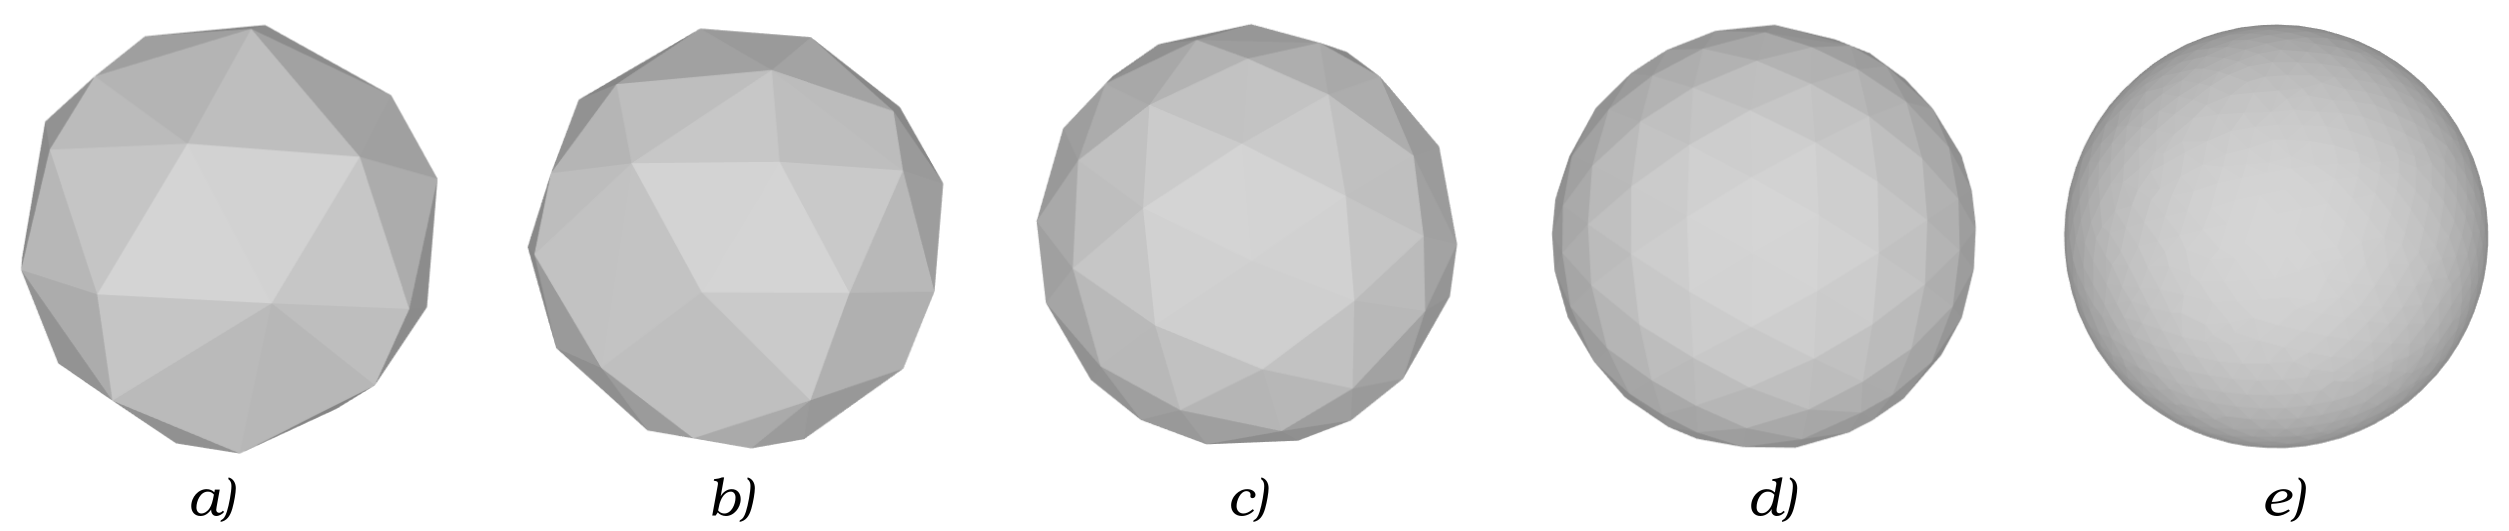
\includegraphics[width=1\textwidth]{images/sphere}}
        \caption[Sféra]{Sféra}
        %id obrazku, pomocou ktoreho sa budeme na obrazok odvolavat
        \label{obr:sphere}
    \end{figure}

    Výsledky meriania kritérii kvality môžeme vidieť v tabuľke \ref{tab:sphere}.
    
    \begin{table}[ht]
    \label{tab:sphere}
    \caption[TODO]{Výsledky merania}
        \begin{center}
            \begin{tabular}{| c |ABCDEFGH|}
                \hline
                \hline
                \multicolumn{9}{|c|}{Sféra} \\
                \hline
                \hline
                $\hspace{5mm} a \hspace{5mm}$ & $k_1$ & $k_2$ & $k_3$ & $k_4$ & $k_5$ & $k_6$ & $k_7$ & $k_8$ \EndTableHeader\\
                \hline
                \hline
                0.9 & 0.506 & 0.085 & 0.725 & 0.9 & 0.506 & 0.085 & 0.725 & 0.726 \\
                \hline
                0.7 & 0.612 & 0.079 & 0.798 & 0.9 & 0.506 & 0.085 & 0.725 & 0.726\\
                \hline
                0.5 & 0.679 & 0.062 & 0.846 & 0.9 & 0.506 & 0.085 & 0.725 & 0.726\\
                \hline
                0.3 & 0.778 & 0.041 & 0.895 & 0.9 & 0.506 & 0.085 & 0.725 & 0.726 \\
                \hline
                0.1 & 0.892 & 0.015 & 0.954 & 0.9 & 0.506 & 0.085 & 0.725 & 0.726\\
                \hline
                \hline
            \end{tabular}
        \end{center}
    \end{table}

}

\newpage

\item{
    \textit{Elipsoid}
    \begin{equation}
    \label{eq:ellipsoid}
        \bigg ( \frac{x-1}{2} \bigg )^2 + \bigg (\frac{y-1}{3} \bigg )^2 + (z - 1)^2 - 1 = 0
    \end{equation}

    Na obrázku \ref{obr:ellipsoid} vidíme výslednú trianguláciu elipsoidu daného implicitnou 
    rovnicou \ref{eq:ellipsoid} s piatimi rôznymi dĺžkami strany $a$.
    \begin{enumerate}[a)]
    \item{
        $a=0.9$, $n=214$, $p=$
    }
    \item{
        $a=0.7$, $n=332$, $p=$
    }
    \item{
        $a=0.5$, $n=574$, $p=$
    }
    \item{
        $a=0.3$, $n=1460$, $p=$
    }
    \item{
        $a=0.15$, $n=5476$, $p=$
    }
    \end{enumerate}

    \begin{figure}
        \centerline{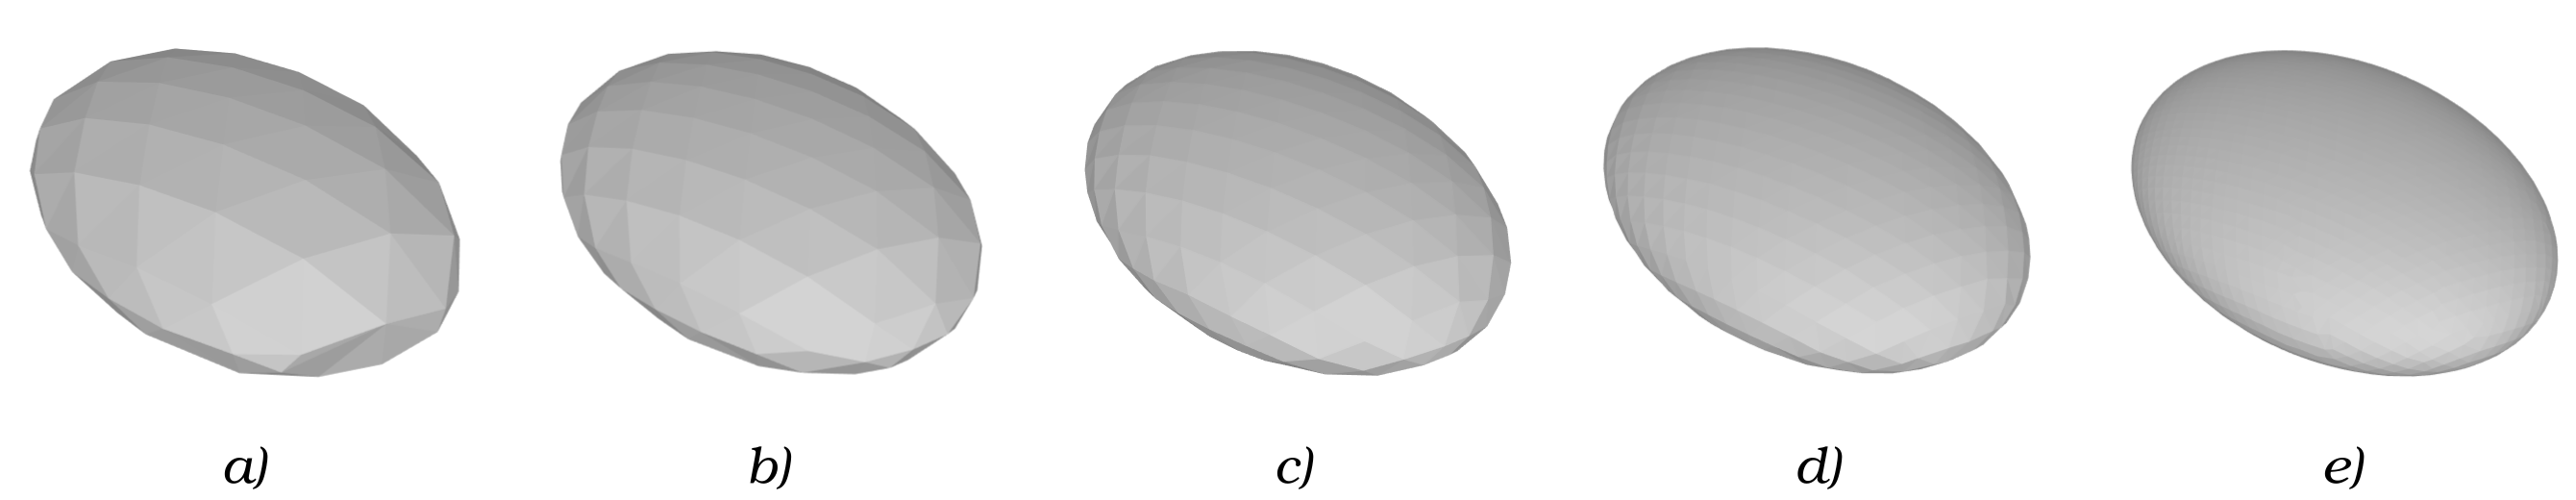
\includegraphics[width=1\textwidth]{images/ellipsoid}}
        \caption[Elipsoid]{Elipsoid}
        %id obrazku, pomocou ktoreho sa budeme na obrazok odvolavat
        \label{obr:ellipsoid}
    \end{figure}

    Výsledky meriania kritérii kvality môžeme vidieť v tabuľke \ref{tab:ellipsoid}.

     
%\renewcommand*{\MinNumberC}{0.8}%
%\renewcommand*{\MidNumberC}{0.9}%
%\renewcommand*{\MaxNumberC}{1.0}%
  

    \begin{table}[ht]
    \label{tab:ellipsoid}
    \caption[TODO]{Výsledky merania}
        \begin{center}
            \begin{tabular}{|c|A B C D E F G H|}
                \hline
                \hline
                \multicolumn{9}{|c|}{Elipsoid} \\
                \hline
                \hline
                $\hspace{5mm} a \hspace{5mm}$ & $k_1$ & $k_2$ & $k_3$ & $k_4$ & $k_5$ & $k_6$ & $k_7$ & $k_8$ \EndTableHeader\\
                \hline
                \hline
                0.9 & 0.629 & 0.049 & 0.802 & 0.9 & 0.629 & 0.049 & 0.802 & 0.802 \\
                \hline
                0.7 & 0.680 & 0.041 & 0.828 & 0.9 & 0.629 & 0.049 & 0.802 & 0.802\\
                \hline
                0.5 & 0.777 & 0.035 & 0.885 & 0.9 & 0.629 & 0.049 & 0.802 & 0.802\\
                \hline
                0.3 & 0.854 & 0.024 & 0.930 & 0.9 & 0.629 & 0.049 & 0.802 & 0.802\\
                \hline
                0.15 & 0.915 & 0.013 & 0.962 & 0.9 & 0.629 & 0.049 & 0.802 & 0.802\\
                \hline
                \hline
            \end{tabular}
        \end{center}
    \end{table}
}


\newpage

\item{
    \textit{Zaoblená kocka}
    \begin{equation}
    \label{eq:cubed_sphere}
        x^4+y^4+z^4-1 = 0
    \end{equation}

    Na obrázku \ref{obr:cubed_sphere} vidíme výslednú trianguláciu zaoblenej kocky danej implicitnou 
    rovnicou \ref{eq:cubed_sphere} s piatimi rôznymi dĺžkami strany $a$.
    \begin{enumerate}[a)]
    \item{
        $a=2$, $n=30$, $p=$
    }
    \item{
        $a=1$, $n=68$, $p=$
    }
    \item{
        $a=0.5$, $n=216$, $p=$
    }
    \item{
        $a=0.25$, $n=748$, $p=$
    }
    \item{
        $a=0.15$, $n=2034$, $p=$
    }
    \end{enumerate}

    \begin{figure}
        \centerline{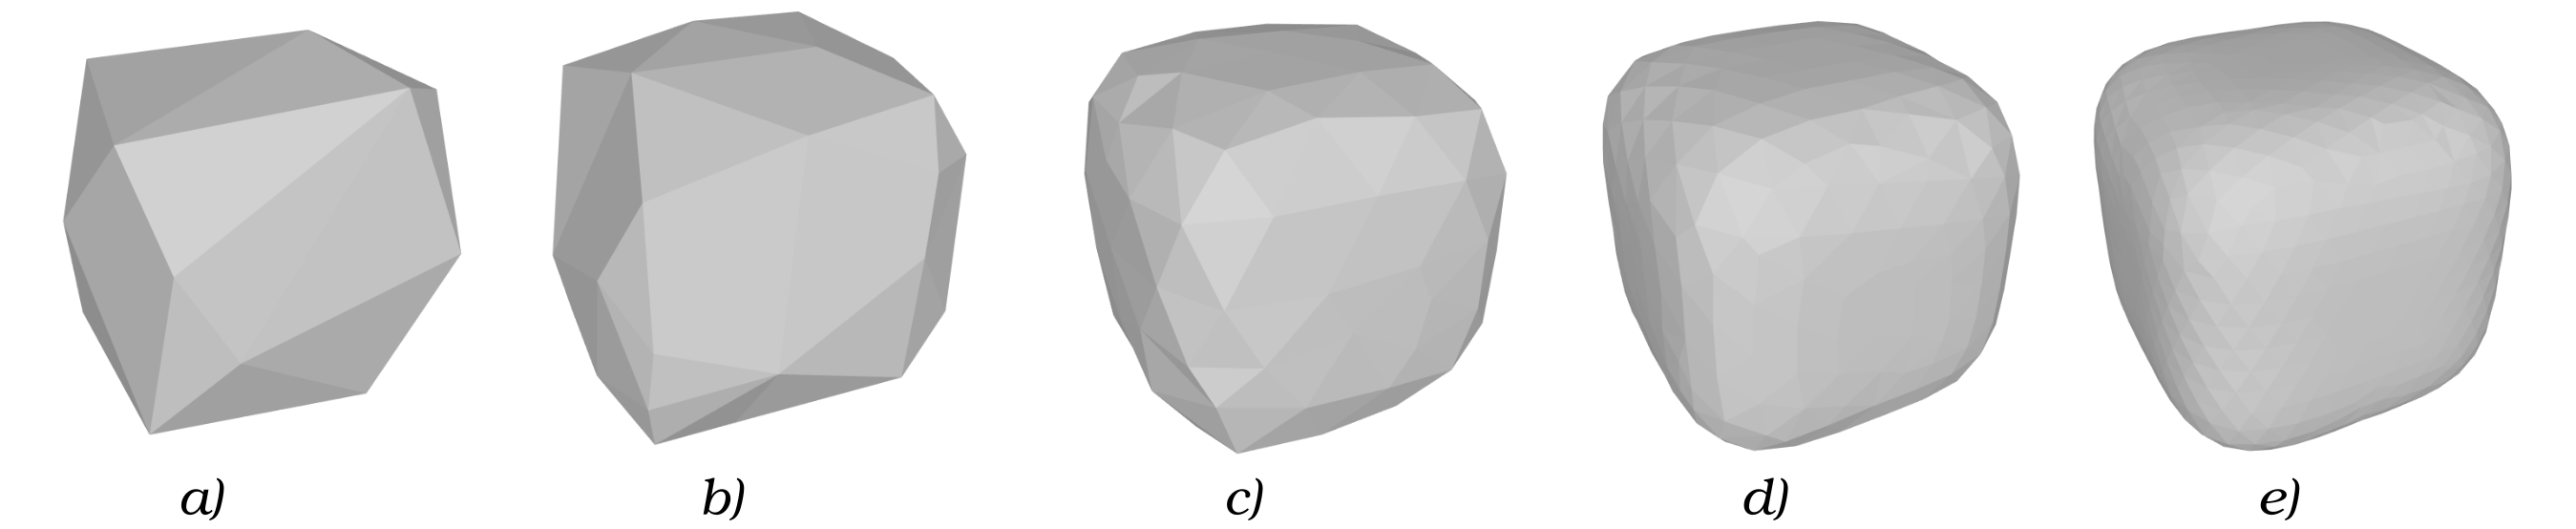
\includegraphics[width=1\textwidth]{images/cubed_sphere}}
        \caption[Zaoblená kocka]{Zaoblená kocka}
        %id obrazku, pomocou ktoreho sa budeme na obrazok odvolavat
        \label{obr:cubed_sphere}
    \end{figure}

    Výsledky meriania kritérii kvality môžeme vidieť v tabuľke \ref{tab:cubed_sphere}.

    
     \begin{table}[ht]
     \label{tab:cubed_sphere}
     \caption[]{Výsledky merania}
        \begin{center}
            \begin{tabular}{|c|A B C D E F G H|}
                \hline
                \hline
                \multicolumn{9}{|c|}{Zaoblená kocka} \\
                \hline
                \hline
                $\hspace{5mm} a \hspace{5mm}$ & $k_1$ & $k_2$ & $k_3$ & $k_4$ & $k_5$ & $k_6$ & $k_7$ & $k_8$ \EndTableHeader\\
                \hline
                \hline
                2 & 0.281 & 0.066 & 0.555 & 0.9 & 0.629 & 0.049 & 0.802 & 0.802\\
                \hline
                1 & 0.541 & 0.077 & 0.750 & 0.9 & 0.629 & 0.049 & 0.802 & 0.802\\
                \hline
                0.5 & 0.727 & 0.051 & 0.865 & 0.9 & 0.629 & 0.049 & 0.802 & 0.802\\
                \hline
                0.25 & 0.860 & 0.031 & 0.935 & 0.9 & 0.629 & 0.049 & 0.802 & 0.802\\
                \hline
                0.15 & 0.885 & 0.020 & 0.949 & 0.9 & 0.629 & 0.049 & 0.802 & 0.802\\
                \hline
                \hline
            \end{tabular}
        \end{center}
    \end{table}
}

\newpage

\item{
    \textit{Torus}
    \begin{equation}
    \label{eq:torus}
        (x^2+y^2+z^2+1375)^2-6400(x^2+y^2) = 0
    \end{equation}

    Na obrázku \ref{obr:torus} vidíme výslednú trianguláciu torusu daného implicitnou 
    rovnicou \ref{eq:torus} s piatimi rôznymi dĺžkami strany $a$.
    \begin{enumerate}[a)]
    \item{
        $a=15$, $n=334$, $p=$
    }
    \item{
        $a=12$, $n=494$, $p=$
    }
    \item{
        $a=9$, $n=818$, $p=$
    }
    \item{
        $a=6$, $n=1720$, $p=$
    }
    \item{
        $a=3$, $n=6596$, $p=$
    }
    \end{enumerate}

    \begin{figure}
        \centerline{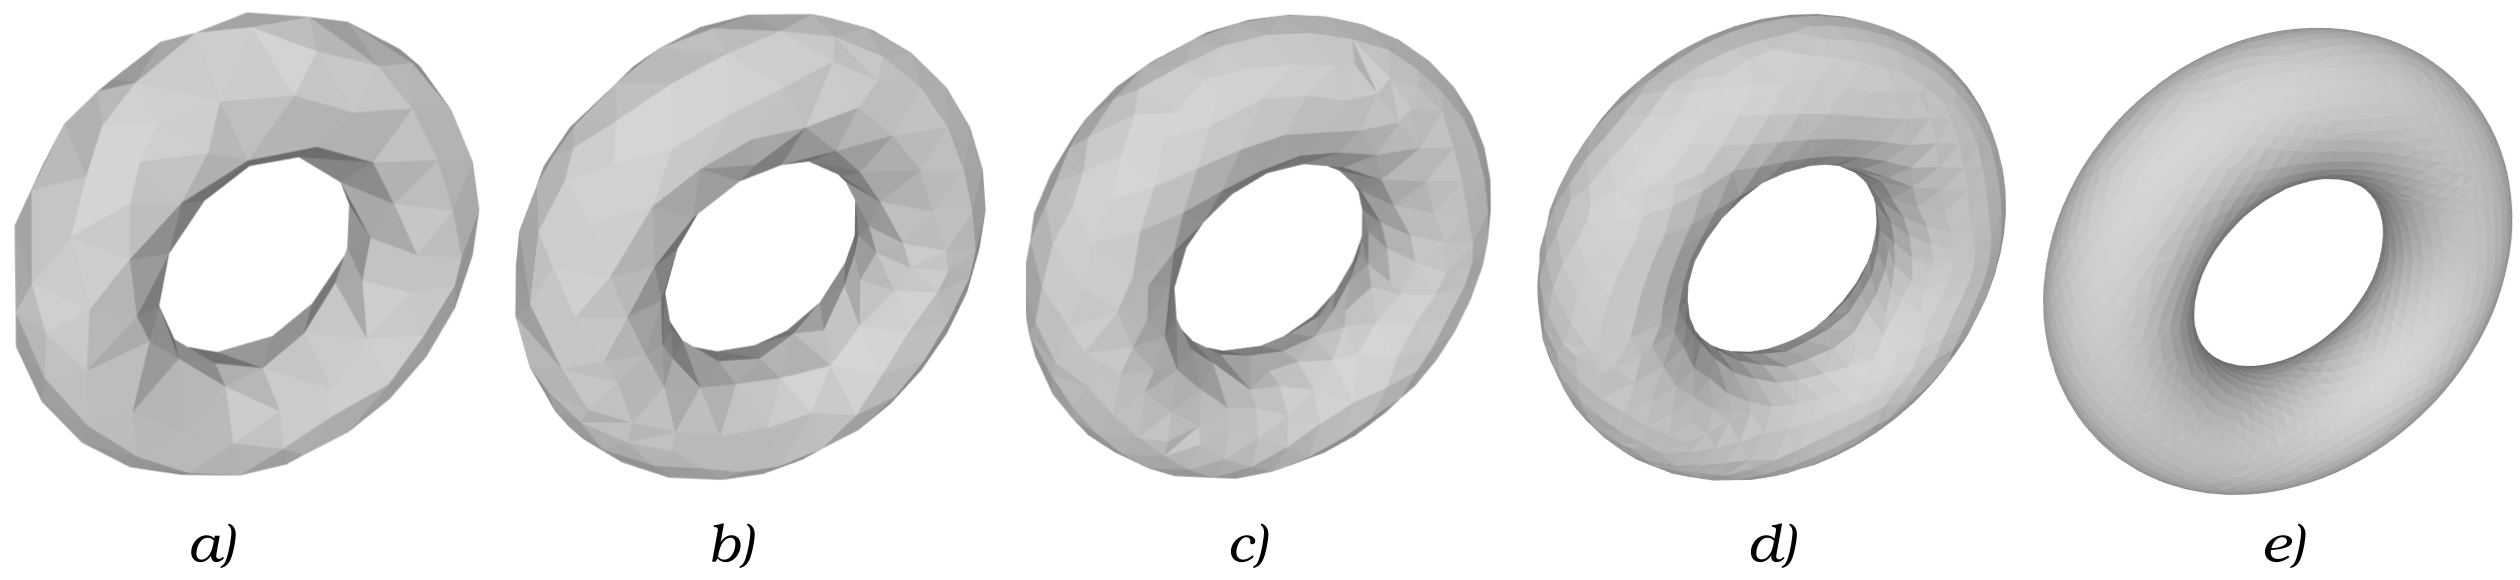
\includegraphics[width=1\textwidth]{images/torus}}
        \caption[Torus]{Torus}
        %id obrazku, pomocou ktoreho sa budeme na obrazok odvolavat
        \label{obr:torus}
    \end{figure}

    Výsledky meriania kritérii kvality môžeme vidieť v tabuľke \ref{tab:torus}.

     
%\renewcommand*{\MinNumberC}{0.8}%
%\renewcommand*{\MidNumberC}{0.9}%
%\renewcommand*{\MaxNumberC}{1.0}%
  
     \begin{table}[ht]
     \label{tab:torus}
     \caption[TODO]{Výsledky merania}
        \begin{center}
            \begin{tabular}{|c|A B C D E F G H|}
                \hline
                \hline
                \multicolumn{9}{|c|}{Torus} \\
                \hline
                \hline
                $\hspace{5mm} a \hspace{5mm}$ & $k_1$ & $k_2$ & $k_3$ & $k_4$ & $k_5$ & $k_6$ & $k_7$ & $k_8$ \EndTableHeader\\
                \hline
                \hline
                15 & 0.710 & 0.060 & 0.856 & 0.9 & 0.629 & 0.049 & 0.802 & 0.802\\
                \hline
                12 & 0.756 & 0.051 & 0.882 & 0.9 & 0.629 & 0.049 & 0.802 & 0.802\\
                \hline
                9 & 0.817 & 0.042 & 0.916 & 0.9 & 0.629 & 0.049 & 0.802 & 0.802\\
                \hline
                6 & 0.879 & 0.030 & 0.946 & 0.9 & 0.629 & 0.049 & 0.802 & 0.802\\
                \hline
                3 & 0.921 & 0.015 & 0.968 & 0.9 & 0.629 & 0.049 & 0.802 & 0.802\\
                \hline
                \hline
            \end{tabular}
        \end{center}
    \end{table}

}

\newpage

\item{
    \textit{Genus}
    \begin{equation}
    \label{eq:genus}
        (x^2+y^2+z^2+1375)^2-6400(x^2+y^2) = 0
    \end{equation}

    Na obrázku \ref{obr:genus} vidíme výslednú trianguláciu torusu daného implicitnou 
    rovnicou \ref{eq:genus} s piatimi rôznymi dĺžkami strany $a$.
    \begin{enumerate}[a)]
    \item{
        $a=15$, $n=334$, $p=$
    }
    \item{
        $a=12$, $n=494$, $p=$
    }
    \item{
        $a=9$, $n=818$, $p=$
    }
    \item{
        $a=6$, $n=1720$, $p=$
    }
    \item{
        $a=3$, $n=6596$, $p=$
    }
    \end{enumerate}

    \begin{figure}
        \centerline{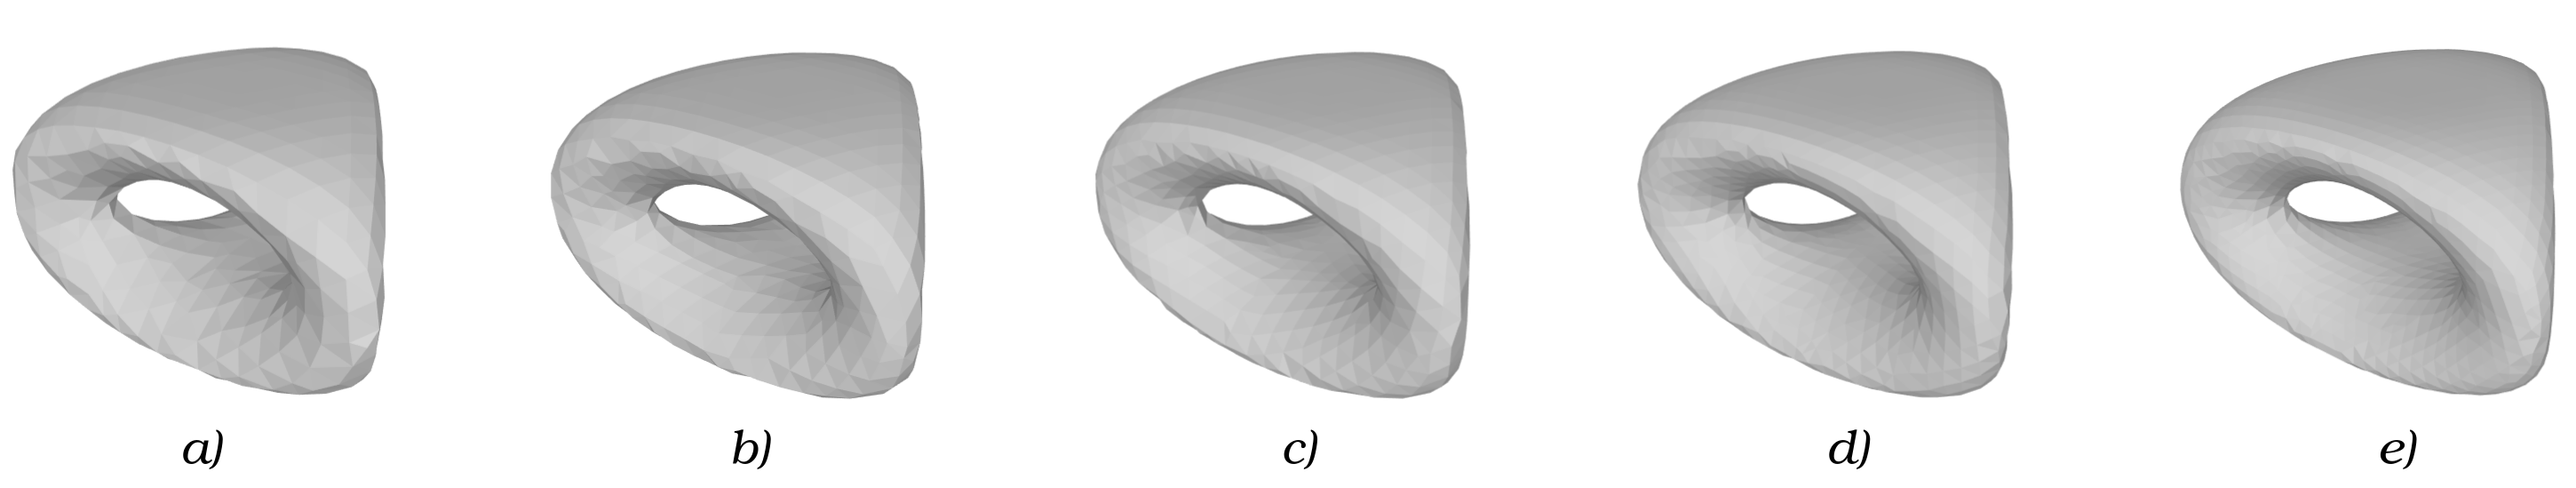
\includegraphics[width=1\textwidth]{images/genus}}
        \caption[Genus]{Genus}
        %id obrazku, pomocou ktoreho sa budeme na obrazok odvolavat
        \label{obr:genus}
    \end{figure}

    Výsledky meriania kritérii kvality môžeme vidieť v tabuľke \ref{tab:genus}.

    \begin{table}[ht]
     \label{tab:genus}
     \caption[TODO]{Výsledky merania}
        \begin{center}
            \begin{tabular}{|c|A B C D E F G H|}
                \hline
                \multicolumn{9}{|c|}{Genus} \\
                \hline
                $\hspace{5mm} a \hspace{5mm}$ & $k_1$ & $k_2$ & $k_3$ & $k_4$ & $k_5$ & $k_6$ & $k_7$ & $k_8$ \EndTableHeader\\
                \hline
                0.225 & 0.808 & 0.029 & 0.912 & 0.9 & 0.629 & 0.049 & 0.802 & 0.802\\
                \hline
                0.2 & 0.819 & 0.027 & 0.918 & 0.9 & 0.629 & 0.049 & 0.802 & 0.802\\
                \hline
                0.175 & 0.845 & 0.024 & 0.931 & 0.9 & 0.629 & 0.049 & 0.802 & 0.802\\
                \hline
                0.15 & 0.858 & 0.021 & 0.937 & 0.9 & 0.629 & 0.049 & 0.802 & 0.802\\
                \hline
                0.125 & 0.892 & 0.018 & 0.954 & 0.9 & 0.629 & 0.049 & 0.802 & 0.802\\
                \hline
                \hline
            \end{tabular}
        \end{center}
    \end{table}

}
\newpage

\item{
    \textit{Tetrahedron}
    \begin{equation}
    \label{eq:tetrahedron}
        (x^2+y^2+z^2+1375)^2-6400(x^2+y^2) = 0
    \end{equation}

    Na obrázku \ref{obr:tetrahedron} vidíme výslednú trianguláciu torusu daného implicitnou 
    rovnicou \ref{eq:tetrahedron} s piatimi rôznymi dĺžkami strany $a$.
    \begin{enumerate}[a)]
    \item{
        $a=15$, $n=334$, $p=$
    }
    \item{
        $a=12$, $n=494$, $p=$
    }
    \item{
        $a=9$, $n=818$, $p=$
    }
    \item{
        $a=6$, $n=1720$, $p=$
    }
    \item{
        $a=3$, $n=6596$, $p=$
    }
    \end{enumerate}

    \begin{figure}
        \centerline{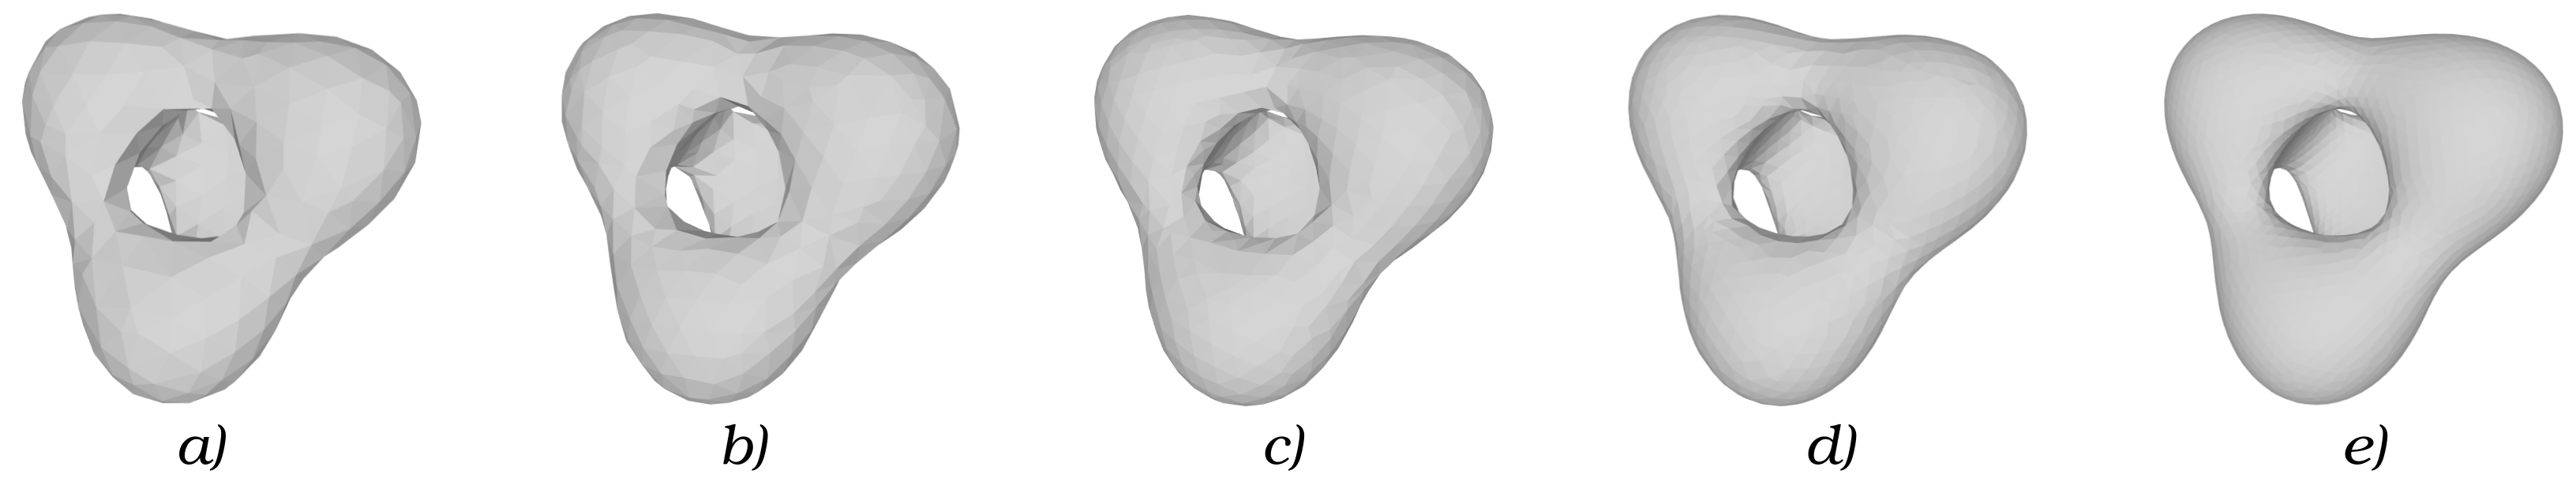
\includegraphics[width=1\textwidth]{images/tetrahedron}}
        \caption[Tetrahedron]{Tetrahedron}
        %id obrazku, pomocou ktoreho sa budeme na obrazok odvolavat
        \label{obr:tetrahedron}
    \end{figure}

    Výsledky meriania kritérii kvality môžeme vidieť v tabuľke \ref{tab:tetrahedron}.

    \begin{table}[ht]
     \label{tab:tetrahedron}
     \caption[TODO]{Výsledky merania}
        \begin{center}
            \begin{tabular}{|c|A B C D E F G H|}
                \hline
                \multicolumn{9}{|c|}{Tetrahedron} \\
                \hline
                $\hspace{5mm} a \hspace{5mm}$ & $k_1$ & $k_2$ & $k_3$ & $k_4$ & $k_5$ & $k_6$ & $k_7$ & $k_8$ \EndTableHeader\\
                \hline
                0.225 & 0.808 & 0.029 & 0.912 & 0.9 & 0.629 & 0.049 & 0.802 & 0.802\\
                \hline
                0.2 & 0.819 & 0.027 & 0.918 & 0.9 & 0.629 & 0.049 & 0.802 & 0.802\\
                \hline
                0.175 & 0.845 & 0.024 & 0.931 & 0.9 & 0.629 & 0.049 & 0.802 & 0.802\\
                \hline
                0.15 & 0.858 & 0.021 & 0.937 & 0.9 & 0.629 & 0.049 & 0.802 & 0.802\\
                \hline
                0.125 & 0.892 & 0.018 & 0.954 & 0.9 & 0.629 & 0.049 & 0.802 & 0.802\\
                \hline
                \hline
            \end{tabular}
        \end{center}
    \end{table}

}
 
\item{
    \textit{Blobby}
    \begin{equation}
    \label{eq:blobby}
        (x^2+y^2+z^2+1375)^2-6400(x^2+y^2) = 0
    \end{equation}

    Na obrázku \ref{obr:blobby} vidíme výslednú trianguláciu torusu daného implicitnou 
    rovnicou \ref{eq:blobby} s piatimi rôznymi dĺžkami strany $a$.
    \begin{enumerate}[a)]
    \item{
        $a=15$, $n=334$, $p=$
    }
    \item{
        $a=12$, $n=494$, $p=$
    }
    \item{
        $a=9$, $n=818$, $p=$
    }
    \item{
        $a=6$, $n=1720$, $p=$
    }
    \item{
        $a=3$, $n=6596$, $p=$
    }
    \end{enumerate}

    \begin{figure}
        \centerline{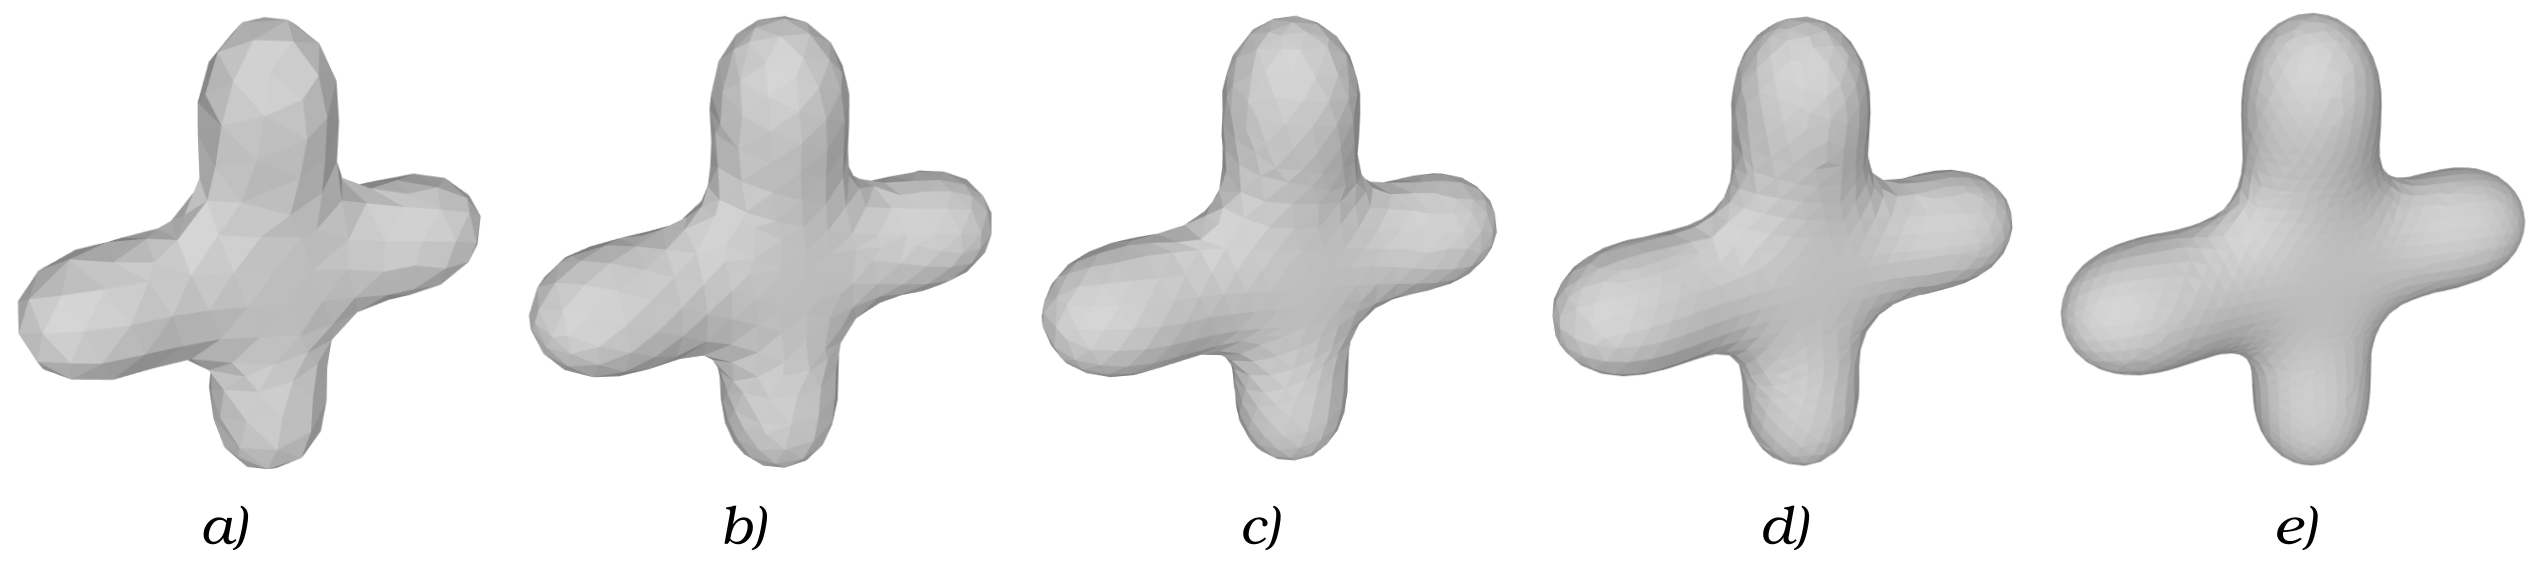
\includegraphics[width=1\textwidth]{images/blobby}}
        \caption[Blobby]{Blobby}
        %id obrazku, pomocou ktoreho sa budeme na obrazok odvolavat
        \label{obr:blobby}
    \end{figure}

    Výsledky meriania kritérii kvality môžeme vidieť v tabuľke \ref{tab:tetrahedron}.

    \begin{table}[ht]
     \label{tab:blobby}
     \caption[TODO]{Výsledky merania}
        \begin{center}
            \begin{tabular}{|c|A B C D E F G H|}
                \hline
                \multicolumn{9}{|c|}{Blobby} \\
                \hline
                $\hspace{5mm} a \hspace{5mm}$ & $k_1$ & $k_2$ & $k_3$ & $k_4$ & $k_5$ & $k_6$ & $k_7$ & $k_8$ \EndTableHeader\\
                \hline
                0.225 & 0.808 & 0.029 & 0.912 & 0.9 & 0.629 & 0.049 & 0.802 & 0.802\\
                \hline
                0.2 & 0.819 & 0.027 & 0.918 & 0.9 & 0.629 & 0.049 & 0.802 & 0.802\\
                \hline
                0.175 & 0.845 & 0.024 & 0.931 & 0.9 & 0.629 & 0.049 & 0.802 & 0.802\\
                \hline
                0.15 & 0.858 & 0.021 & 0.937 & 0.9 & 0.629 & 0.049 & 0.802 & 0.802\\
                \hline
                0.125 & 0.892 & 0.018 & 0.954 & 0.9 & 0.629 & 0.049 & 0.802 & 0.802\\
                \hline
                \hline
            \end{tabular}
        \end{center}
    \end{table}

}
\item{
    \textit{Osem-sféra}
    \begin{equation}
    \label{eq:joined_spheres}
        (x^2+y^2+z^2+1375)^2-6400(x^2+y^2) = 0
    \end{equation}

    Na obrázku \ref{obr:joined_spheres} vidíme výslednú trianguláciu torusu daného implicitnou 
    rovnicou \ref{eq:joined_spheres} s piatimi rôznymi dĺžkami strany $a$.
    \begin{enumerate}[a)]
    \item{
        $a=15$, $n=334$, $p=$
    }
    \item{
        $a=12$, $n=494$, $p=$
    }
    \item{
        $a=9$, $n=818$, $p=$
    }
    \item{
        $a=6$, $n=1720$, $p=$
    }
    \item{
        $a=3$, $n=6596$, $p=$
    }
    \end{enumerate}

    \begin{figure}
        \centerline{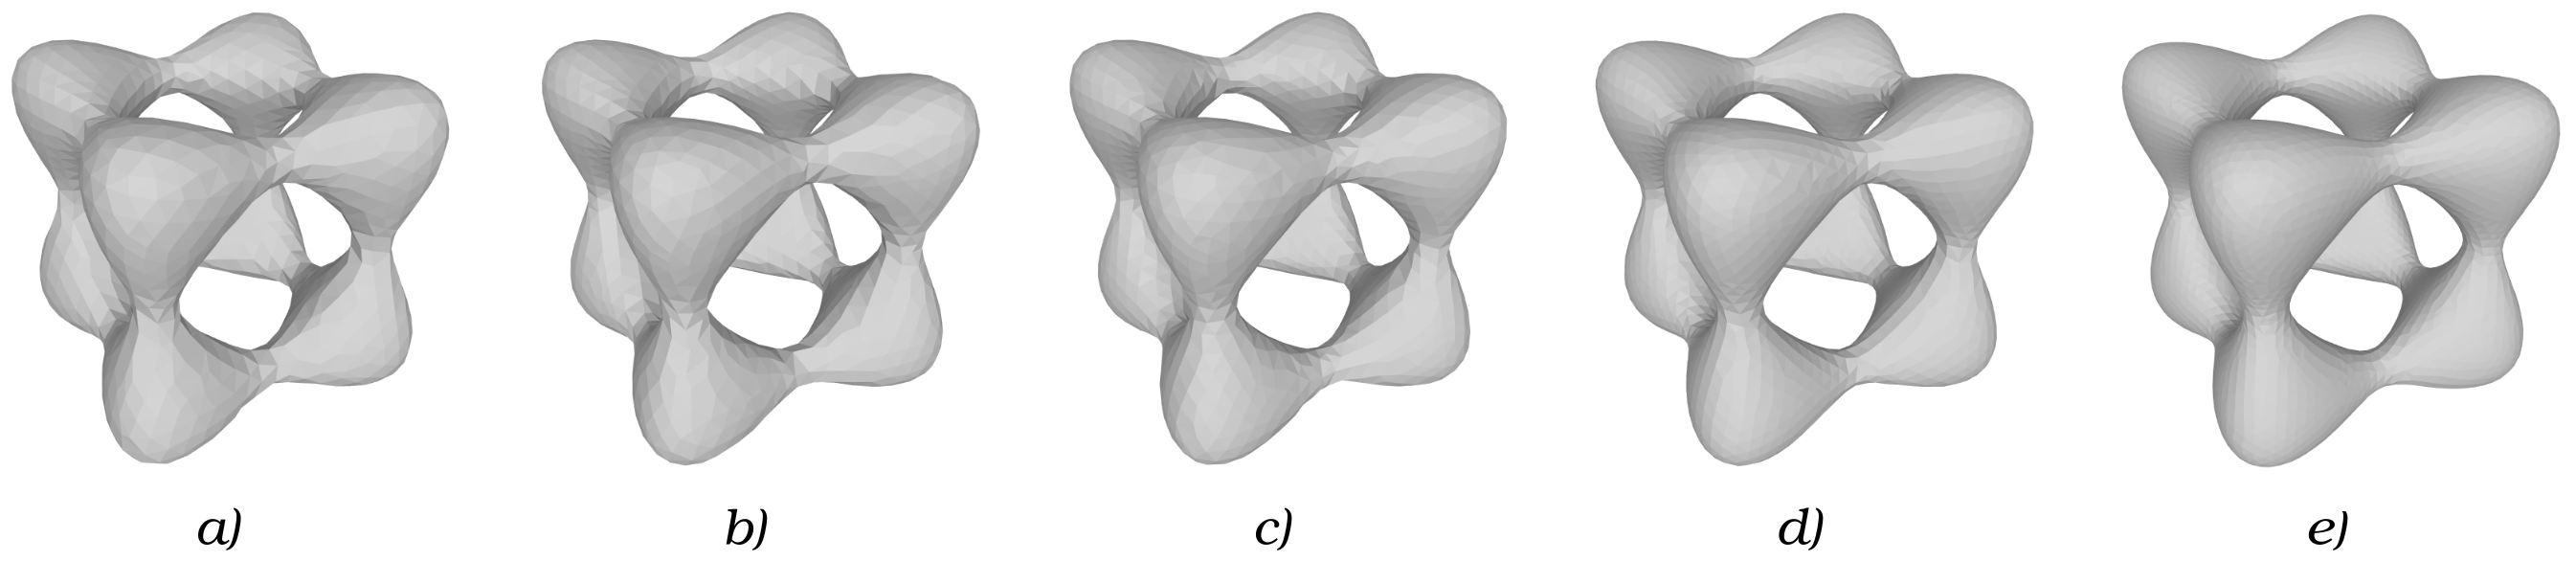
\includegraphics[width=1\textwidth]{images/joined_spheres}}
        \caption[Osem-sféra]{Osem-sféra}
        %id obrazku, pomocou ktoreho sa budeme na obrazok odvolavat
        \label{obr:joined_spheres}
    \end{figure}

    Výsledky meriania kritérii kvality môžeme vidieť v tabuľke \ref{tab:joined_spheres}.

    \begin{table}[ht]
     \label{tab:joined_spheres}
     \caption[TODO]{Výsledky merania}
        \begin{center}
            \begin{tabular}{|c|A B C D E F G H|}
                \hline
                \multicolumn{9}{|c|}{Osem-sféra} \\
                \hline
                $\hspace{5mm} a \hspace{5mm}$ & $k_1$ & $k_2$ & $k_3$ & $k_4$ & $k_5$ & $k_6$ & $k_7$ & $k_8$ \EndTableHeader\\
                \hline
                0.225 & 0.808 & 0.029 & 0.912 & 0.9 & 0.629 & 0.049 & 0.802 & 0.802\\
                \hline
                0.2 & 0.819 & 0.027 & 0.918 & 0.9 & 0.629 & 0.049 & 0.802 & 0.802\\
                \hline
                0.175 & 0.845 & 0.024 & 0.931 & 0.9 & 0.629 & 0.049 & 0.802 & 0.802\\
                \hline
                0.15 & 0.858 & 0.021 & 0.937 & 0.9 & 0.629 & 0.049 & 0.802 & 0.802\\
                \hline
                0.125 & 0.892 & 0.018 & 0.954 & 0.9 & 0.629 & 0.049 & 0.802 & 0.802\\
                \hline
                \hline
            \end{tabular}
        \end{center}
    \end{table}

}
     

\end{enumerate}

TODO opísať pozorovania

\section{Nekonečné plochy}

V tejto kapitole odprezentujeme výsledky dosiahnuté pri triangulácii plôch s použítím 
ohraničujúcej obálky. Ohraničujúcu obálku máme zadanú ako $3$-rozmerný interval 
$\langle x_{min}, x_{max}\rangle
\times \langle y_{min}, y_{max}\rangle \times \langle z_{min}, z_{max}\rangle \in \mathbb{R}^3.$ 




    
     \begin{table}[ht]
        \begin{center}
            \begin{tabular}{|c|A B C D E F G H|}
                \hline
                \multicolumn{9}{|c|}{Genus} \\
                \hline
                $\hspace{5mm} a \hspace{5mm}$ & $k_1$ & $k_2$ & $k_3$ & $k_4$ & $k_5$ & $k_6$ & $k_7$ & $k_8$ \EndTableHeader\\
                \hline
                0.225 & 0.808 & 0.029 & 0.912 & 0.9 & 0.629 & 0.049 & 0.802 & 0.802\\
                \hline
                0.2 & 0.819 & 0.027 & 0.918 & 0.9 & 0.629 & 0.049 & 0.802 & 0.802\\
                \hline
                0.175 & 0.845 & 0.024 & 0.931 & 0.9 & 0.629 & 0.049 & 0.802 & 0.802\\
                \hline
                0.15 & 0.858 & 0.021 & 0.937 & 0.9 & 0.629 & 0.049 & 0.802 & 0.802\\
                \hline
                0.125 & 0.892 & 0.018 & 0.954 & 0.9 & 0.629 & 0.049 & 0.802 & 0.802\\
                \hline
                \hline
            \end{tabular}
        \end{center}
    \end{table}

    
     \begin{table}[ht]
        \begin{center}
            \begin{tabular}{|c|A B C D E F G H|}
                \hline
                \multicolumn{9}{|c|}{Blobby} \\
                \hline
                $\hspace{5mm} a \hspace{5mm}$ & $k_1$ & $k_2$ & $k_3$ & $k_4$ & $k_5$ & $k_6$ & $k_7$ & $k_8$ \EndTableHeader\\
                \hline
                0.2 & 0.751 & 0.051 & 0.881 & 0.9 & 0.629 & 0.049 & 0.802 & 0.802\\
                \hline
                0.15 & 0.792 & 0.039 & 0.901 & 0.9 & 0.629 & 0.049 & 0.802 & 0.802\\
                \hline
                0.12 & 0.855 & 0.034 & 0.935 & 0.9 & 0.629 & 0.049 & 0.802 & 0.802 \\
                \hline
                0.1 & 0.870 & 0.028 & 0.943 & 0.9 & 0.629 & 0.049 & 0.802 & 0.802\\
                \hline
                0.07 & 0.909 & 0.021 & 0.962 & 0.9 & 0.629 & 0.049 & 0.802 & 0.802\\
                \hline
                \hline
            \end{tabular}
        \end{center}
    \end{table}

    \begin{table}[ht]
        \begin{center}
            \begin{tabular}{|c|A B C D E F G H|}
                \hline
                \multicolumn{9}{|c|}{Tetrahedron} \\
                \hline
                $\hspace{5mm} a \hspace{5mm}$ & $k_1$ & $k_2$ & $k_3$ & $k_4$ & $k_5$ & $k_6$ & $k_7$ & $k_8$ \EndTableHeader\\
                \hline
                0.6 & 0.757 & 0.040 & 0.885 & 0.9 & 0.629 & 0.049 & 0.802 & 0.802\\
                \hline
                0.5 & 0.793 & 0.034 & 0.903 & 0.9 & 0.629 & 0.049 & 0.802 & 0.802\\
                \hline
                0.4 & 0.818 & 0.028 & 0.917 & 0.9 & 0.629 & 0.049 & 0.802 & 0.802\\
                \hline
                0.3 & 0.861 & 0.022 & 0.940 & 0.9 & 0.629 & 0.049 & 0.802 & 0.802\\
                \hline
                0.2 & 0.915 & 0.015 & 0.966 & 0.9 & 0.629 & 0.049 & 0.802 & 0.802\\
                \hline
                \hline
            \end{tabular}
        \end{center}
    \end{table}


    \begin{table}[ht]
        \begin{center}
            \begin{tabular}{|c|A B C D E F G H|}
                \hline
                \multicolumn{9}{|c|}{Osem-guľa} \\
                \hline
                $\hspace{5mm} a \hspace{5mm}$ & $k_1$ & $k_2$ & $k_3$ & $k_4$ & $k_5$ & $k_6$ & $k_7$ & $k_8$ \EndTableHeader\\
                \hline
                0.3 & 0.807 & 0.036 & 0.911 & 0.9 & 0.629 & 0.049 & 0.802 & 0.802\\
                \hline
                0.275 & 0.815 & 0.033 & 0.915 & 0.9 & 0.629 & 0.049 & 0.802 & 0.802\\
                \hline
                0.25 & 0.833 & 0.031 & 0.924 & 0.9 & 0.629 & 0.049 & 0.802 & 0.802\\
                \hline
                0.2 & 0.870 & 0.026 & 0.943 & 0.9 & 0.629 & 0.049 & 0.802 & 0.802\\
                \hline
                0.15 & 0.903 & 0.020 & 0.960 & 0.9 & 0.629 & 0.049 & 0.802 & 0.802\\
                \hline
                \hline
            \end{tabular}
        \end{center}
    \end{table}


    %The min, mid and max values
    %\renewcommand{\MinNumberA}{0.2}%
    %\renewcommand{\MidNumberA}{0.6} %
    %\renewcommand{\MaxNumberA}{1.0}%